\documentclass{article}
\usepackage{shortex}
\usepackage[margin=1in]{geometry}
\usepackage{listings}
\usepackage{xcolor}
% \usepackage{jupynotex}
\usepackage{csvsimple}
\usepackage{placeins}
% \usepackage{hyperref}
\usepackage{subcaption}
\usepackage{algorithm}
\usepackage{algpseudocode}
\usepackage{booktabs}
\usepackage{colortbl}


\graphicspath{{./graphics}}

\lstdefinelanguage{Julia}{
    keywords={function, end, if, else, elseif, for, while, return, 
               local, global, const, struct, mutable, abstract, type,
               using, import, export, module, begin, let, do, try, 
               catch, finally, true, false, nothing},
    sensitive=true,
    comment=[l]{\#},
    morecomment=[s]{\#=}{=\#},
    morestring=[b]",
    morestring=[b]',
}

\lstset{
    language=Julia,
    basicstyle=\ttfamily\small,
    keywordstyle=\color{blue}\bfseries,
    commentstyle=\color{gray}\itshape,
    stringstyle=\color{purple},
    numberstyle=\tiny\color{gray},
    numbers=left,
    stepnumber=1,
    frame=single,
    breaklines=true,
    captionpos=b,
    tabsize=4,
    showstringspaces=false,
}

\lstset{
    literate={ρ}{$\rho$}{1}
             {α}{$\alpha$}{1}
             {β}{$\beta$}{1}
             {σ}{$\sigma$}{1}
             {σ²}{$\sigma^2$}{2}
             {μ}{$\mu$}{1}
             {ϵ}{$\epsilon$}{1}
             {η}{$\eta$}{1}
             {η²}{{$\eta^2$}}{2}
             {r̂}{$\hat r$}{1}
             {Δ}{$\Delta$}{1}
             {Λ}{$\Lambda$}{1}
             {∞}{$\infty$}{1}
}

\begin{document}
\title{STAT 547E - Report - Diffusion Schrödinger Bridge}
\author{Zachary Lau}
\date{\today}
\maketitle

\begin{abstract}
The Schrödinger Bridge problem is a classic problem in physics, which has
received renewed attention in statistics thanks to its application to diffusion
models, and from recent mathematical work in optimal transport. This report
provides an accessible introduction to the Schrödinger bridge problem for
statisticians, discusses its connection to diffusion models, and provides a
simple MCMC algorithm to sample from a finite particle approximation.  Our
particle approximation method implicitly regularizes for entropy via the
aggregation from microstats to macrostates. Preliminary experimental evidence
shows reasonable ability of our algorithm to approximate the static Schrödinger
bridge solution in moderate dimensions, although further work is
needed to understand scaling limits and tuning parameters.  \end{abstract}

\section{Introduction}
Recent work in generative modelling has brought particular focus to the area
of diffusion processes
\cite{ho2020denoisingdiffusionprobabilisticmodels}
\cite{song2020generativemodelingestimatinggradients}. Amongst these works,
\cite{debortoli2023diffusionschrodingerbridgeapplications}
makes use of the concept of a Schrödinger bridge
\cite{Schrodinger1932}; a diffusion process with
constrained marginals that ensures finite time transitions from the data
distribution to the prior.

This report builds up intuition about the Schrödinger bridge problem from the
ground up, based on a finite particle perspective.
We begin with discussing Brownian bridges, the fundamental building blocks of
the Schrödinger bridge.  We then move onto mixtures of Brownian bridges which
arise when we have multiple pairs of particles. By allowing the particles'
pairings to be chosen probabilistically according to the diffusion dynamics, we
recover a finite version of the Schrödinger bridge problem. In the limit of
infinite particles, this approaches exactly the standard Schrödinger bridge
problem.

In addition to introducing the problem formulation, we discuss the classical
Sinkhorn solution, as well as the novel generative modelling centered
formulation provided by DeBortoli et al
\cite{debortoli2023diffusionschrodingerbridgeapplications}.  Finally we
introduce a simple MCMC algorithm to simulate from the finite particle system,
and graphically demonstrate the simulations consistency with the 
Schrödinger bridge problem. Numerical experiments show that our solution
performs well when the number of particles is sufficiently larger relative to
the dimension of the problem, or there is sufficient Brownian noise.

\section{Background}
\subsection{Brownian Bridges}
The Brownian Bridge can be seen as the precursor problem of the Schrödinger
Bridge Problem. The set up is as follows.  Consider a particle that begins at point $X_0
= 0$ at time $t=0$. This particle evolves according to a standard Brownian
motion (e.g. Wiener process with unit variance). Then conditioning on the
starting position, the location of the particle at time $t$ is given by 
\begin{align}
    X_t|X_0 = 0 \sim \Norm(0, t)
\end{align}
Now additionally consider observing $X_1 = 0$. Conditioning on both $X_0 = 0$
and $X_1 = 0$, the distribution of $X_t$ can be found analytically. Based on the
Markovian property of the Brownian motion, $X_1 | X_t \sim \Norm(X_t, 1-t)$.
In other words $X_1 = X_t - (1-t) Z$ where $Z \sim \Norm(0,1)$ is drawn
independently of $X_t$. This gives $\Cov(X_t, X_1) = \Var(X_t) = t$, and hence
we recover the joint distribution 
\begin{align}
    X_t, X_1 | X_0 = 0 \sim \Norm\left( 
        \begin{bmatrix} 0 \\ 0 \end{bmatrix},
        \begin{bmatrix}
            t & t \\
            t & 1
        \end{bmatrix}
    \right)
\end{align}
Now conditioning on $X_1 = 0$ as well, we find
\begin{align}
    X_t | X_1 = 0, X_t = 0 \sim \Norm(0, t(1-t))
\end{align}
Here we derive the variance from the Schur complement, or equivalently simply
from the properties of multivariate Gaussians. Considering all $t$
simultaneously, this is known as a Brownian bridge. This result is quite
aesthetic, we note that it is symmetric, which reflects the symmetry in Brownian
motion.  Furthermore as Schrödinger points out in his original paper, the
density can be seen as a \emph{product} of a density term from a Brownian motion
starting at $X_0=0$ and another time-reversed Brownian motion starting at
$X_1=0$. As a minor extension, if we instead consider a particle starting at
$X_0=a$ and ending at $X_1=b$, we get the intermediary distributions
\begin{align}
    X_t | X_0 = a, X_1 = b \sim \Norm(ta + (1-t)b, t(1-t))
\end{align}
In other words, we have simply added a linear drift term. 
% TODO - do we talk about the corresponding SDE?

\subsection{Brownian Bridges - Multiple Independent Particles}
We next consider a system of $N$ particles, each independently undergoing
Brownian motion. Suppose that we know the starting and ending point of each
particle. We use superscripts to denote particle indices. That is we know
$X^1_0 = a_1, X^2_0 = a_2, \ldots, X^1_1 = b_1, X^2_1 = b_2, \ldots$. Each
particle independently traverses a Brownian bridge from its starting point to
its end point. That is
\begin{align}
    X^i_t | X^i_0 = a_i, X^i_1 = b_i \sim \Norm(ta_i + (1-t)b_i, t(1-t))
\end{align}
Looking at the particles as a collective, we might be
concerned with the overall \emph{density} of particles at time $t$. This 
density is given by a \emph{mixture of normals} defined by the respective
Brownian Bridges.

\subsection{Unknown Pairings - A Bayesian Perspective}
\label{sec:unknown}
Next we will generalize further. Suppose that we observe the locations of the
$N$ particles at the beginning and the end, but we don't know which particle
corresponds to which! How can we pair the particles? We will take an approach
that is a hybrid of statistical mechanics and Bayesian inference. First we place
a \emph{uniform prior} on all possible pairings. Then we consider conditioning
on the \emph{difference} between the start and the end points, that is we 
condition on $X^i_1 - X^i_0$. We note that we have to work with differences
because we haven't fully specified a probability model; the Brownian motion only
specifies the relationship between $X_1$ and $X_0$. This gives a Gaussian
likelihood $\mathcal L \propto \exp\left(-\frac 1 2(x_1-x_0)^2\right)$. Denoting
the pairing by the tuple of vectors $(\mathbf i, \mathbf j)$ and, 
taking this product over all $i$ points, we get the posterior over pairings by
\begin{align}
    p(\mathbf i,\mathbf j) \propto \prod_{(i,j)} \exp\left(-\frac 1 2(a_i-b_j)^2\right)
\end{align}
(To ensure the pairing is uniquely identifiable we may fix $\mathbf i = [1, 2,
3, \ldots, N]$). We make an interesting physical remark that will become
important later. Supposing that we associated $q$ with the counting measure on
$[N] \times [N]$ where $[n] = \{1, \ldots N\}$ such that $q(i,j)=\frac 1 N$ if
the particle that starts at $i$ ends up at location $j$ and $0$ otherwise (i.e.
it absorbs all the information about which particle goes where). Let
$r$ be the reference measure on $[N] \times [N]$ given by
$r(i,j) = \exp\left(-\frac 1 2(a_i-b_j)^2\right)$. Then $r$ contains all the
information about how Brownian motion actually works (i.e. about the underlying
system). It is typically not normalized. The log posterior turns out to be the
negative cross-entropy between $q$ and $r$. That is
\begin{align}
    -H(q,r) &= \int \log r(i,j) \d q \\
    &= \frac 1 N \sum_{(i,j)} -\frac 1 2 (a_i - b_j)^2 \\
    &= \frac 1 N \log p(\mathbf i, \mathbf j) \\
    \log p(\mathbf i, \mathbf j) &= -NH(q,r)
\end{align}
Already, we can see some interesting phenomena. Firstly, we notice the
similarity between the sum of squares losses and the cost function in the
Monge-Kantorovich problem. We will return to this later. Furthermore, notice
that multiplying the log-likelihood by $N$ corresponds to a sort of \emph{power
posterior}. Therefore for large $N$ we might expect the posterior to concentrate
near the minimizer of the cross-entropy.

\subsection{Many particles, finite points}
\label{sec:many_particles}
We generalize once more. Let us consider $M$ particles starting at each of
the $N$ locations, for a total of $M \times N$ particles. We need to keep
track of how many particles from each of the $N$ starting locations end up in 
each of the $N$ ending locations. We can easily generalize the discrete measure
$q$ from before such that $q(i,j)$ is the \emph{fraction of particles} starting
at location $i$ and ending up at location $j$. However, now we have to be a
little bit more careful with how we pick our prior. This gets a little confusing
to think of priors over measures, so we introduce another way to think of 
$q$-as a matrix. In this case let the matrix be given by $Q_{i,j} = q(i,j)$.

Firstly we must constrain the support such that the each row and column of 
$Q$ sums to $\frac 1 N$. These are our \emph{marginal} constraints. We next must
consider actually assigning matches between particles on the left and the right.
We again assume a uniform distribution over all possible pairings that respect
our marginal constraints. Note there is a distinction between a uniform 
distribution on pairings and uniform distribution on $Q$
matrices. For example if we swap the labels on two particles we have a new
pairing, but the $Q$ matrix is unchanged! Indeed we have discovered the
difference between a microstate (pairing) and macro-state ($Q$-matrix).

For our $Q$ matrix this has \emph{combinatorial}
implications. The total number of pairings corresponding to a $Q$ matrix is
given by a multinomial, namely
\begin{align}
    \frac{(NM)!}{\prod_{i,j} (NMQ_{i,j})!}
\end{align}
Taking into account
the Brownian Noise likelihood from earlier, we get the posterior
\begin{align}
    p(Q) \propto \frac{1}{\prod_{i,j} (NMQ_{i,j})!}\prod_{(i,j)} \exp\left(-\frac 1 2(a_i-b_j)^2\right) \\
    \log p(Q) = - \sum_{i,j} \log (NMQ_{i,j})! + \sum_{(i,j)} - \frac 1 2 NMQ_{i,j}(a_i - b_j)^2 + \log Z
\end{align}
Where $Z$ is a normalizing constant. Viewing $Q$ as a probability measure, and using $r$
to denote the reference measure from before, the second term becomes a multiple
of the cross entropy, namely $- NM H(q,r)$.
Using Stirling's approximation, the first term becomes 
\begin{align}
    \sum_{i,j} - NMQ_{i,j} \log NMQ_{i,j} + NMQ_{i,j} + O(\log NMQ_{i,j})
\end{align}
On practical scales, the first two terms are the most significant.
Normalizing by the total $NM$ particles,
we note that this approaches the \emph{entropy} (in the statistics sense) of 
$q$ plus a constant
\begin{align}
    \sum_{i,j} -NMQ_{i,j} \log NMQ_{i,j} + NMQ_{i,j} &=
        NM H(q) - NM \log (NM) + NM
\end{align}
Thus our large $M$ approximation gives the posterior as 
\begin{align}
    \log p(Q) &= NM (H(q) - H(q,r)) + NM - NM \log (NM) \\
    &= NM KL(q | r) +  NM - NM \log (NM)
\end{align}
Once again, we see a power posterior. Note that there is another equivalent way we could
have reached this conclusion. First consider $NM$ particles
\emph{unconstrained} by the marginal condition, distributed independently such
that for each particle $P(X_0 = a_i, X_1 = b_j) \propto -\exp\left(-\frac 1 2 (a_i - b_j)^2 \right)$.
The distribution of these particles would correspond exactly to our
\emph{reference} measure from before. If we then \emph{condition} on the marginal
requirements we recover exactly the same posterior! In the nomenclature of
statistical mechanics, the reference measure corresponds to the \emph{energy}
and the distribution over microstates to the \emph{Gibb's distribution}.

Either way we view it, in the limit of infinite $M$, the
distribution on $Q$ collapses to the delta distribution at the minimizer of the
$KL$ to the reference distribution subject to our marginal requirements. In
statistical mechanics we might interpret negative $KL$ as entropy. In other
words, we have discovered the principle of maximum entropy. We have also
discovered the concept of a Schrödinger Bridge. Another interesting point,
we make is to recall that the cross entropy corresponds to the cost function
from the Monge-Kantorovich problem. Thus this optimization problem corresponds
to an \emph{entropy-regularized} version of the Monge-Kantorovich problem,
where the variance of the Brownian motion changes the strength of
regularization.

\subsection{The Schrödinger Bridge Problem}
Armed with a deeper understanding of Brownian bridges, we are now ready to
state the Schrödinger bridge problem as the continuous version of our previous
mixture of Brownian bridges problem. Briefly, given a Riemannian manifold
$\mathcal X$, the (static) Schrödinger bridge problem is to find the joint
distribution $Q$ on $\mathcal X \times \mathcal X$ which
\begin{enumerate}
    \item Satisfies the marginal constraints $X_0 \sim \mu$ and $X_1 \sim \nu$
    \item Minimizes the
KL-divergence to the reference Brownian motion $R$ on $\mathcal X \times \mathcal X$
\end{enumerate}
In the general case, the reference Brownian motion is given by
$R(x_0, x_1) \propto \exp\left(-\frac 1 2 d(x_0, x_1)^2 \right)$. To avoid 
technicalities we may usually take $\mathcal X$ as $\mathbb R^d$. The reference
is always a measure, but it may not be a probability measure. Once
a solution is found, the distribution on paths is just a mixture of
Brownian bridges with weights given by the transport plan.

\subsection{Schrödinger Bridge to Diffusion Models}
Before discussing how to actually compute the Schrödinger bridge, we touch on
why it might be useful for diffusion models. Traditional diffusion models
essentially consist of the following conceptual sequence
\begin{enumerate}
    \item Assume a form for the forward diffusion process with stationary
    distribution at the prior
    \item Run the forward process until it is close to stationary (i.e. the prior)
    \item Use samples from the forward process to \emph{learn} the backwards process.
    This amounts to learning the score
    \cite{ho2020denoisingdiffusionprobabilisticmodels}
    \cite{song2020generativemodelingestimatinggradients}
\end{enumerate}
We might be slightly uncomfortable with the second step above, since it relies
on us simply trusting that the diffusion process has been run long enough.
Solving the Schrödinger bridge problem helps us address this discomfort.
Instead of fixing the forward process and letting it run long enough to reach
stationarity, we can directly find the diffusion process that is closest to
our \emph{reference Brownian motion} while also satisfying the marginal
constraints. This means that we can now force the forward dynamics
to reach the prior \emph{in finite time}, which corresponds to fewer
diffusion steps. This is the
first key idea in \cite{debortoli2023diffusionschrodingerbridgeapplications}.

\subsection{Solving the Schrödinger Bridge Problem}
We now return to the problem of actually solving the Schrödinger bridge problem.
We will focus again on a finite set as discussed in section
\ref{sec:many_particles}. First we will introduce the classic
Sinkhorn algorithm, before moving on to the implementation provided in 
\cite{debortoli2023diffusionschrodingerbridgeapplications}. In our context
the Sinkhorn algorithm is very simple. Let $Q$ be the transport matrix
normalized by the total number of particles. The Sinkhorn algorithm proceeds
as follows
\begin{enumerate}
    \item Initialize $Q$ at the reference distribution
    \item While not converged
    \begin{enumerate}
        \item Rescale the \textbf{rows} to satisfy the row marginal condition
        \item Rescale the \textbf{columns} to satisfy the column marginal condition
        \item Repeat
    \end{enumerate}
\end{enumerate}
It is a remarkable fact shown in \cite{Sinkhorn1964} that this algorithm
converges to the minimum entropy solution which satisfies the marginal
constraints! In fact it can be seen as a version of coordinate ascent in the
\emph{dual} problem. We will not provide a proof of convergence here.

It may be helpful before moving forward to think of this algorithm in terms of
conditional distributions. Let rows correspond to
$X_0$ with target marginal $\mu$ and columns to $X_1$ with target marginal
$\nu$. The very first time we rescale the rows corresponds to computing the joint
distribution specified by $\mu$ and the \emph{reference dynamics}. This joint
distribution implies a \emph{backwards} conditional distribution $X_0|X_1$.
Crucially, if we now reweight the columns, the \emph{backwards} conditional distribution
is maintained and the $X_1$ marginal is adjusted. However, the forward
conditional $X_1 | X_0$ and $X_0$ marginal will now be perturbed. We can
repeat the process, reweighting the $X_0$ marginal and following the new
forward dynamics. The algorithm
will repeat until both marginal constraints are satisfied.

The Sinkhorn algorithm would be perfect if our distributions had finite support.
However, in diffusion modelling we are dealing with \emph{continuous priors},
\emph{high dimensions} and \emph{large datasets} which make a Sinkhorn
discretization infeasible. We could model the potentials using some flexible
parametric family, but finding an appropriate family is a non-trivial problem.
Another solution is to implicitly define the joint distribution by modelling
the \emph{diffusion} process itself. This is the key algorithmic innovation
introduced
in \cite{debortoli2023diffusionschrodingerbridgeapplications}.
At a high-level the algorithm is as follows
\begin{enumerate}
    \item Initialize at the data distribution and use the reference distribution
    for our forward dynamics
    \item Learn the backward dynamics by sampling from the data and propagating
    under the forward dynamics
    \item Learn the forward dynamics by sampling from the prior and
    propagating backwards under our learned backward dynamics
    \item Repeat
\end{enumerate}
This is exactly a continuous analog of the Sinkhorn algorithm, but where
conditional distributions are given by \emph{diffusion dynamics}. Lastly it
is important to note that while we have been using the standard Brownian
motion as our reference distribution, this is only one possible choice. In fact,
each form of the forward SDE corresponds to a \emph{different reference
path distribution} with a different energy function. For example, for the
Variance Preserving SDE \cite{song2021scorebasedgenerativemodelingstochastic}
the corresponding energy function for the static Schrödinger bridge problem
would be $E(i, j) = -\frac 1 2 \frac{(\alpha a_i - b_j)^2}{1-\alpha^2}$ where
$\alpha = \exp\left(-\frac 1 2 \int_0^t \beta(s) \d s\right)$. 

\section{Methodology}
\subsection{Simulation by MCMC}
In section \ref{sec:unknown} we introduced a probability distribution
over transport plans in the finite case. We now introduce a
Markovian interacting particle system which admits this distribution as
a stationary distribution. The introduced distribution can be seen as the
Gibb's distribution, where energy is defined by the reference Brownian motion.
In our case this is proportional to the L2 optimal transport cost. We also
introduce a constant $\epsilon$ which controls the amount of noise in the
Brownian motion, and also hence the trade-off between entropy regularization
and the optimal transport cost function (see figure \ref{fig:epsilon_effect}).
\begin{align}
    p(\mathbf i, \mathbf j) &\propto \exp(-E(\mathbf i, \mathbf j)) \\
    E(\mathbf i, \mathbf j) &= \sum_{(i,j)} -\frac 1 2 \frac{(a_i - b_j)^2}{\epsilon}
\end{align}
The algorithm is described in Algorithm~\ref{alg:bitflip-mh}.
This algorithm is based on Metropolis-Hastings using a combination of
bit-masked swap proposals and random pairings. It alternates between a
\emph{y-swap phase} (swap ending locations) and an \emph{x-swap phase}
(swap starting locations). Each phase sweeps through all $N$ bit indices
proposing swaps of the respective coordinate, then shuffles the indices. The bit
masked swap proposal ensure global communication, while the shuffles break
periodicity. Since energy is summative over all particles, the change in energy
for a proposal can be calculated locally (that is, given only the $a$ and $b$
values of the two interacting particles). The overall kernel can then be seen as
a combination of such local kernels, plus an energy preserving shuffle.

This algorithm approximates the marginal distributions by first independently
sampling the starting and ending points from their desired marginals. Once the
marginal approximations are set, the only moves that are proposed are 
\emph{swap} moves, thus the marginals remain unchanged.  The target is log concave
\cite{léonard2013surveyschrodingerproblemconnections}, therefore multimodality
is not an issue for any sufficiently good MCMC move. An interactive version of the simulation can be
found on
\href{https://zach-lau.github.io/STAT547E-Project/code/particle_sim.html}{Github}
\footnote{\url{https://zach-lau.github.io/STAT547E-Project/code/particle_sim.html}}.
In this 1-dimensional example, $x$ and $y$ locations are deterministically
``sampled'' using the inverse CDF method. This simulation was used to generate
the example in Figure \ref{fig:epsilon_effect} which shows how the Schrödinger
bridge problem interpolates between the independent coupling and the L2
optimal transport plan.

In section \ref{sec:many_particles}, we noted that when such a particle system
includes many particles at the same location, aggregating to macrostates
naturally induces entropy regularization. The setup in this section is
slightly different, in that particles are sampled from the marginals, and thus
not necessarily at exactly the same location. However experimentally and
intuitively sampling from the marginals induces a conceptual \emph{change of measure}
(i.e. from the counting measure to our marginal distribution) which has
the same effect. Future work could focus on formalizing this equivalence in
the asymptotic limit. The key insight is that \emph{aggregating to macrostates
induces entropy regularization}.

While in low dimensions our particle simulation is more of a toy, it may have
real applications as dimensionality scales up. The Sinkhorn algorithm relies
on a discretization of the grid. Naively, such a discretization would
scale \emph{exponentially} in dimension, making it infeasible beyond very
moderate dimensions. Our algorithm on the other hand only requires a sample
from the marginals, which is more tractable in high dimensions.
Furthermore, our MCMC problem is extremely well-behaved; we have a log-concave
target and uniform ergodicity (since we are working on finite state space,
although asymptotic behaviour in the number of particles may warrant closer
study). Moving beyond moderate dimension, it may be possible to integrate this
work with diffusion models by using it to estimate the forward noising model.
That is, given a sample from our data distribution we perform the following steps
\begin{itemize}
    \item Sample an equal-sized distribution from our prior
    \item Pair them using our MCMC algorithm
    \item Noise by interpolating. For example for
the VE-SDE the interpolation is simply the standard Brownian bridge. 
    \item Train a score matching network
\end{itemize}
Under such a scenario, the score
matching network would only need to be trained \emph{once} as opposed to
multiple times as in IMPF
\cite{debortoli2023diffusionschrodingerbridgeapplications}.

\section{Experiments}
We experimentally verify the ability of our method to recover expectations with
respect to the Static Schrödinger bridge problem in the analytically known case
of Gaussians \cite{pmlr-v206-bunne23a}. We consider as our prior a mean-zero
isotropic Gaussian, and as our data distribution a Gaussian with AR(1) structure
for $\rho=0.9$ with mean $\vec e_1$ (that is shifted in the first dimension by
one unit).  We consider dimension $d \in \{10, 30, 100\}$ and the number of
particles $N \in \{100, 1000, 10000\}$. As test functions we use various
functions which depend on the correlation structure induced by the transport
map, since additive functions would simply reflect properties of the marginal
samples and not the transport map itself. We check correlations between
$x_0y_0$, $x_0y_1$, $x_1y_0$ and $x_1y_1$. We also check the first three moments
of the dot product $\vec x \cdot \vec y$. 


For each experiment,
we initially run 1000 iterations to burn-in. After this point, we re-evaluate
each test function after every 10 iterations until we have 1000 measurements
(this can be seen as thinning). From these measurements we can estimate the
distribution of the test function estimates, and compare it to ground truth.
The mean and standard deviation are reported. Furthermore, MSE is presented
relative to ground truth. MSE is broken down into squared bias and variance
based on sample estimates of the first and second moments. Bias is expected
because we are using a finite particle approximation. Because we are not
resampling the marginals, the inaccuracies in the marginals are also lumped into
the bias. Variance is expected because of the variance in the MCMC procedure
itself. We also report estimates of the ESS to contextualize the mean estimates.
Ideally our Monte Carlo Standard Error of the mean (MCSE) will be small relative
to the variance so that the bias variance decomposition is meaningful. 

For now, Claude is tasked with these experiments, including calculating ground
truth values given the analytic expressions found in \cite{pmlr-v206-bunne23a}.
Full results tables are provided in Appendix \ref{sec:experiments}, and code is
available on \href{https://github.com/zach-lau/STAT547E-Project}{Github}
\footnote{\url{https://github.com/zach-lau/STAT547E-Project}}. These results
indicate that the particle approximation is able to perform well when the number
of particles is sufficiently larger relative to the dimension, and when there is
sufficient Brownian noise. However, it struggles somewhat with estimating higher
moments (e.g. third moments). The MSE is dominated by the bias term. This term
includes the influence of the initial conditions, including the random
initialization of the marginals.  Based on these results, future experimental
work may focus on resampling the marginals, as well as diagnostics for
checking convergence. From the relative size of the
bias and variance in the current regime, we conjecture that for accurate
estimates the Markov chains only needs to be run until stationarity. After this
point, there is little benefit to be had from running further, and that it
would be more advantageous to simply add more particles, or resample the particle
locations themselves, such as with a local move that accounts for both the energy
difference as well as the marginal density. It is important to note
that many chains have very low ESS, but the general variance bias breakdown is
consistent across all chains, including both those with high and low ESS. 

\begin{figure}[ht]
    \centering
    \begin{subfigure}[t]{0.32\textwidth}
        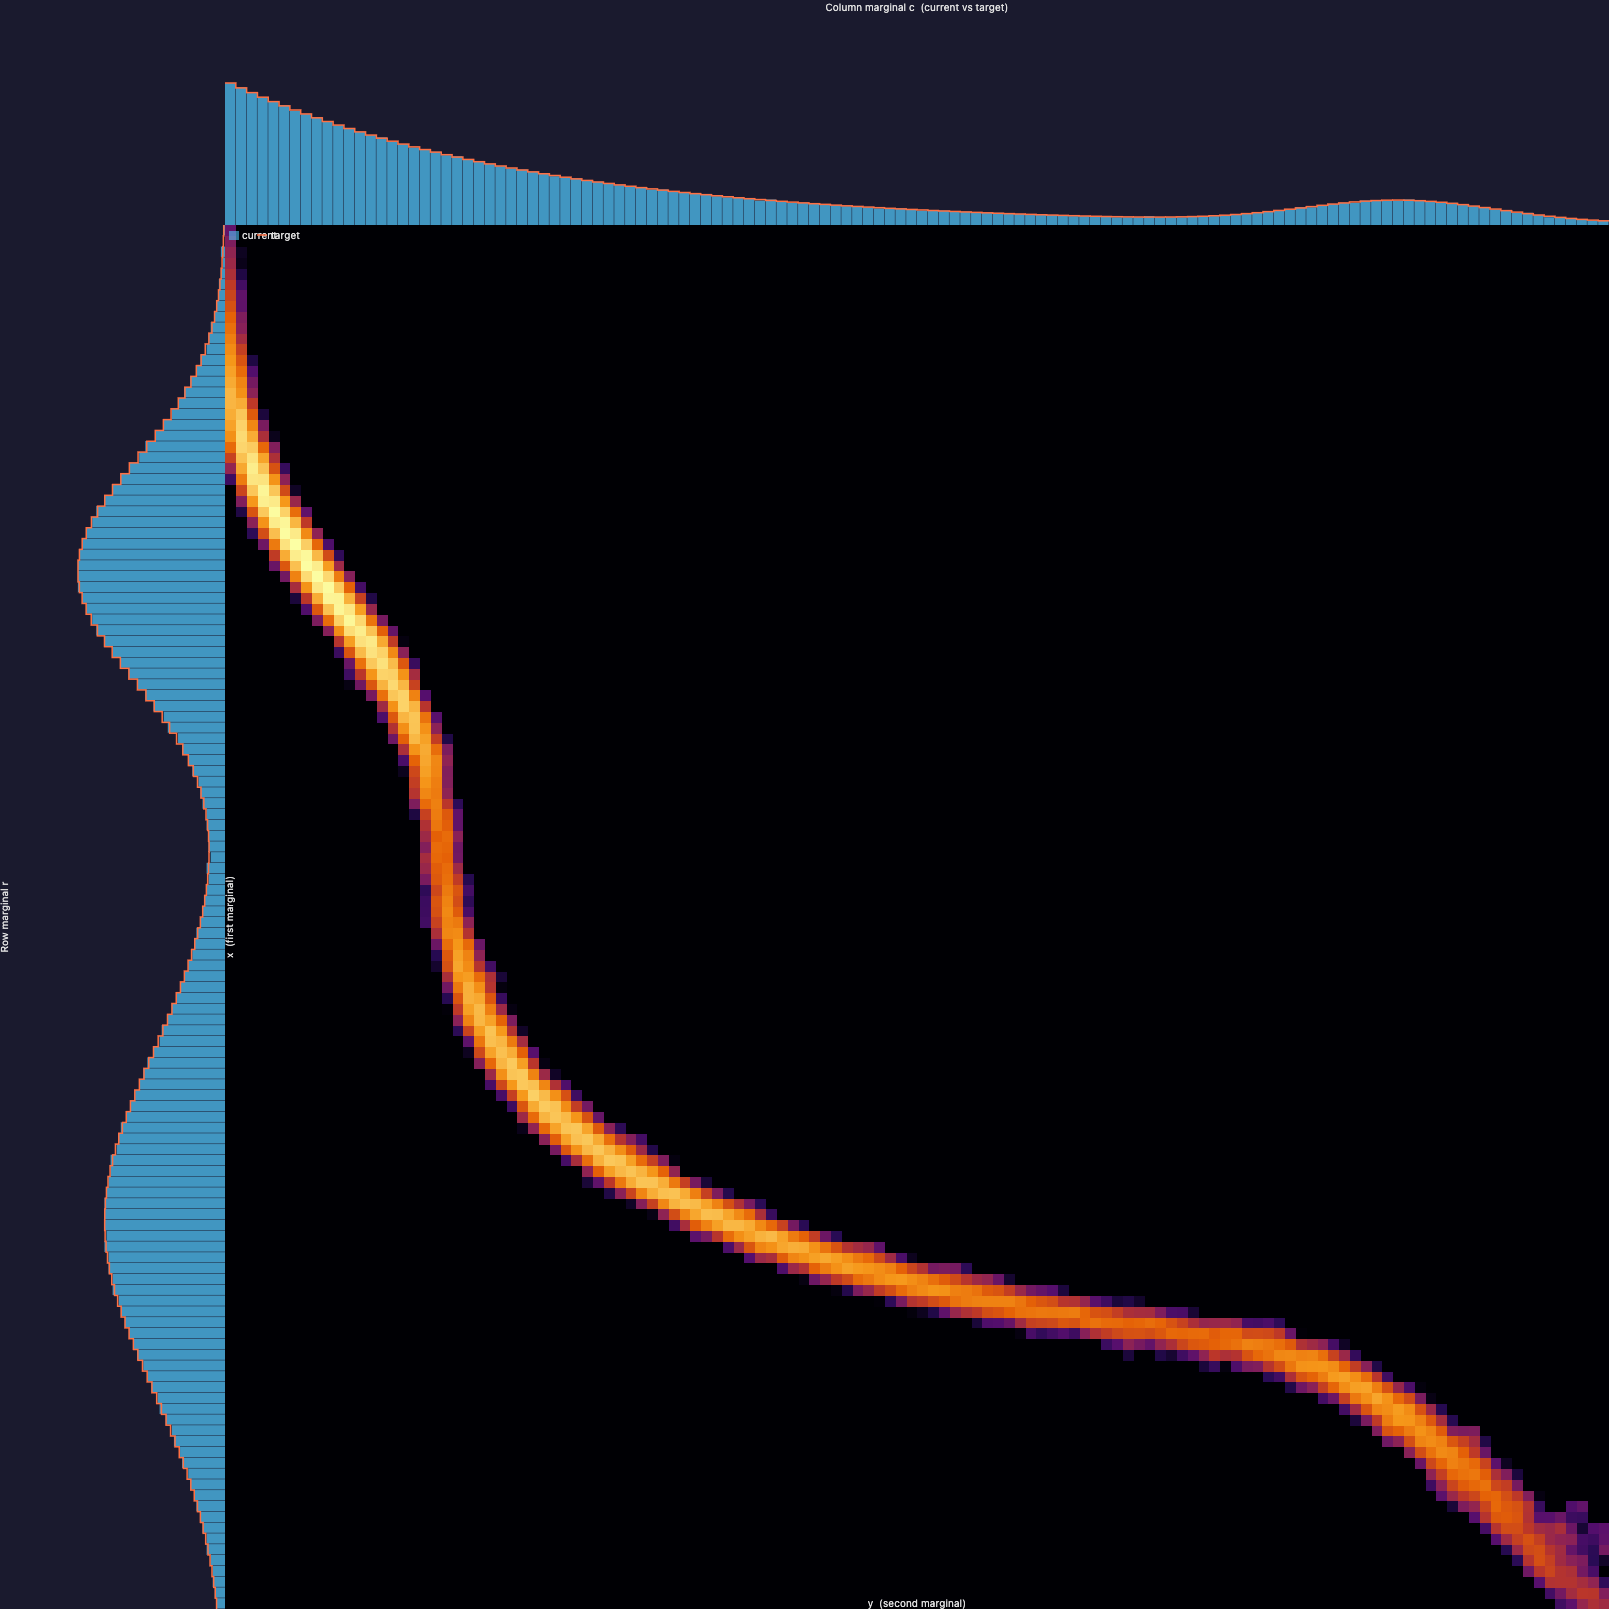
\includegraphics[width=\textwidth]{../graphics/OT.png}
        \caption{Low temperature ($\varepsilon \to 0$): recovers the deterministic optimal transport map.}
        \label{fig:ot}
    \end{subfigure}
    \hfill
    \begin{subfigure}[t]{0.32\textwidth}
        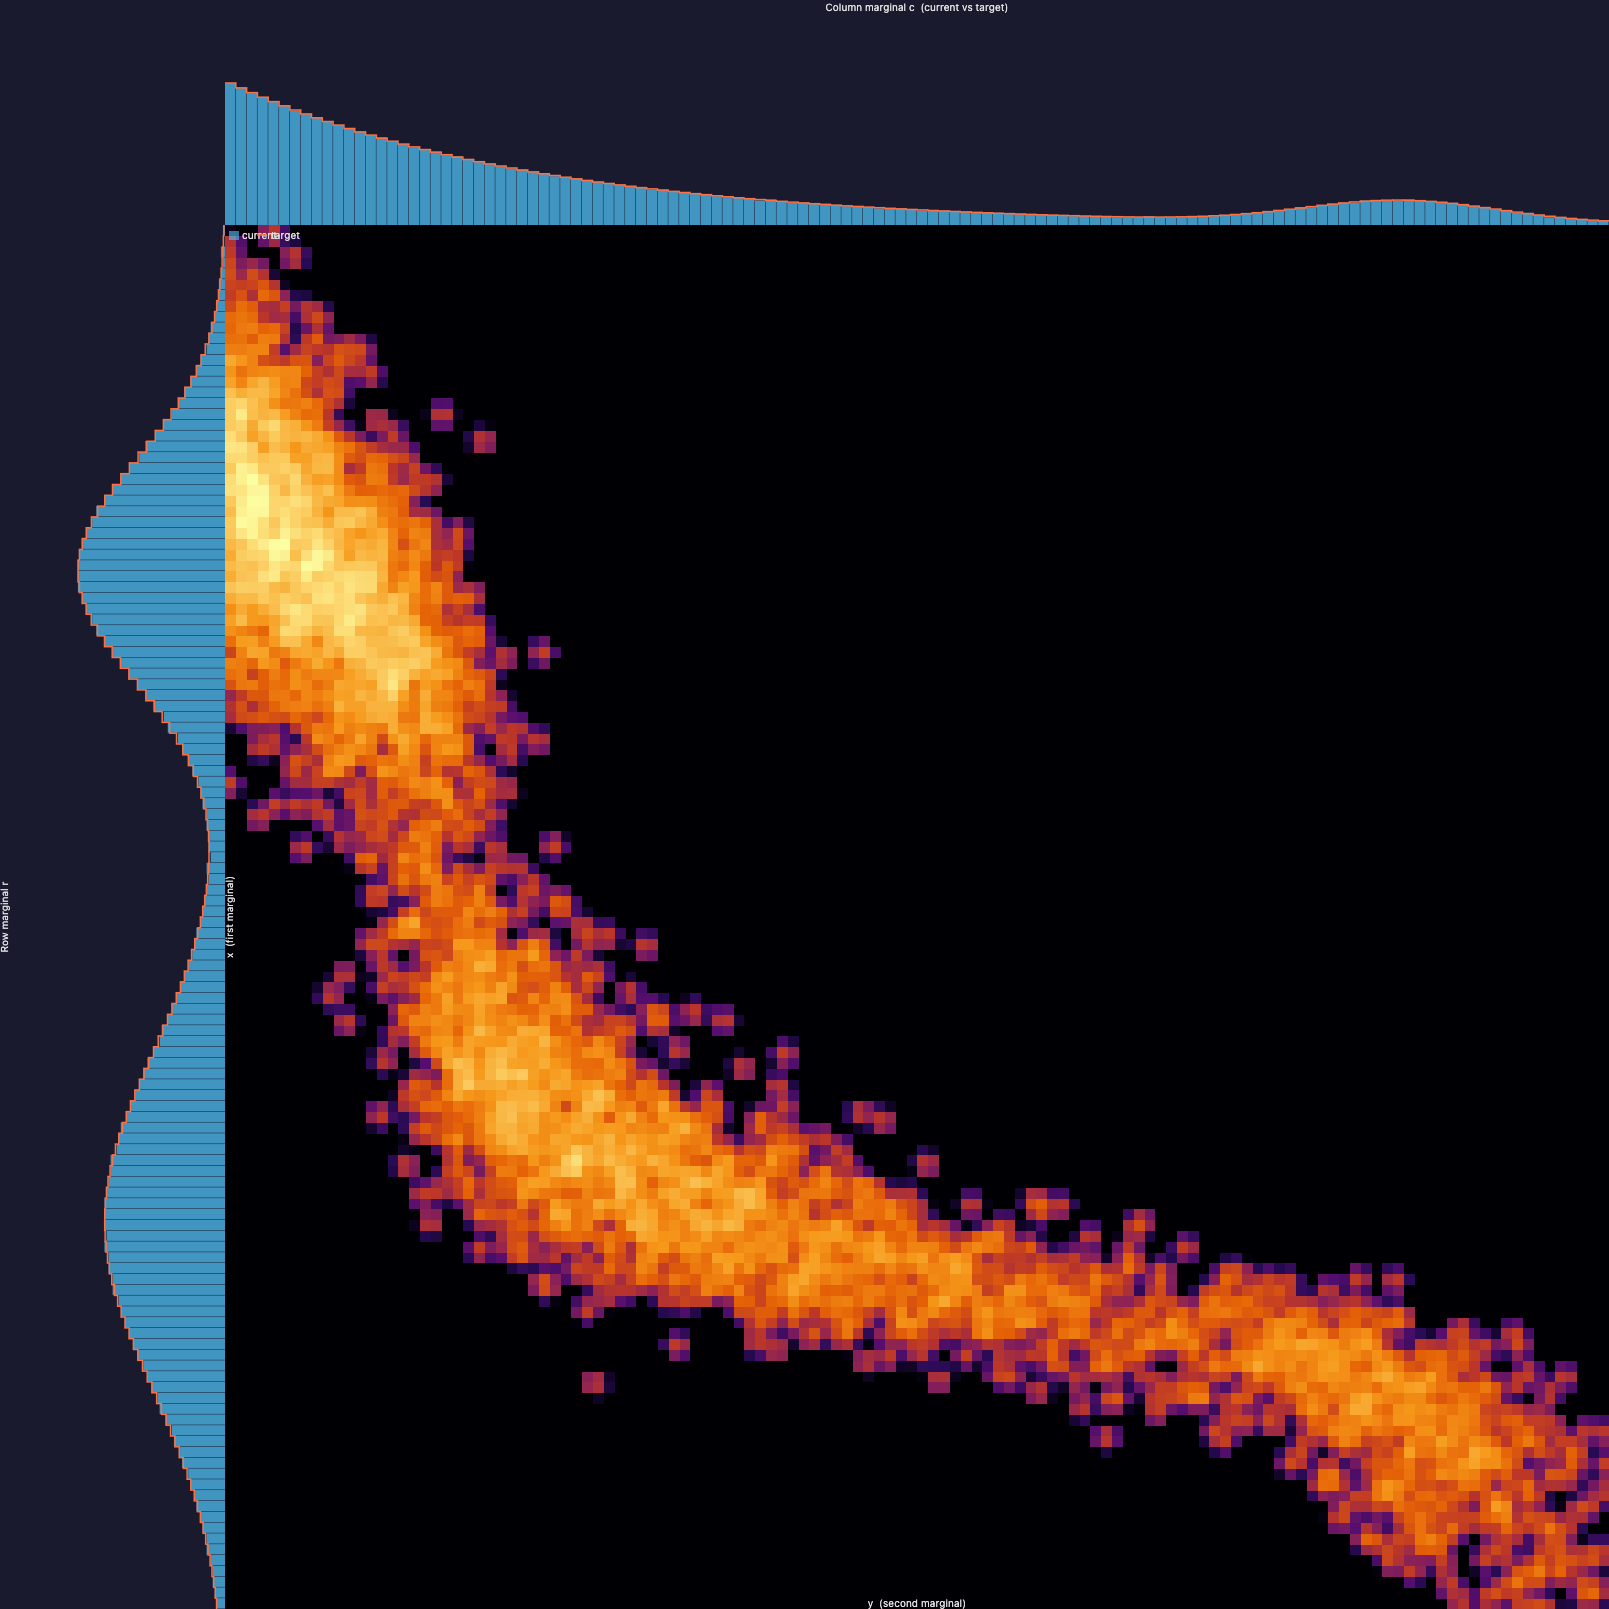
\includegraphics[width=\textwidth]{../graphics/sb.png}
        \caption{Moderate temperature: the Schr\"{o}dinger bridge, a stochastic transport plan.}
        \label{fig:sb}
    \end{subfigure}
    \hfill
    \begin{subfigure}[t]{0.32\textwidth}
        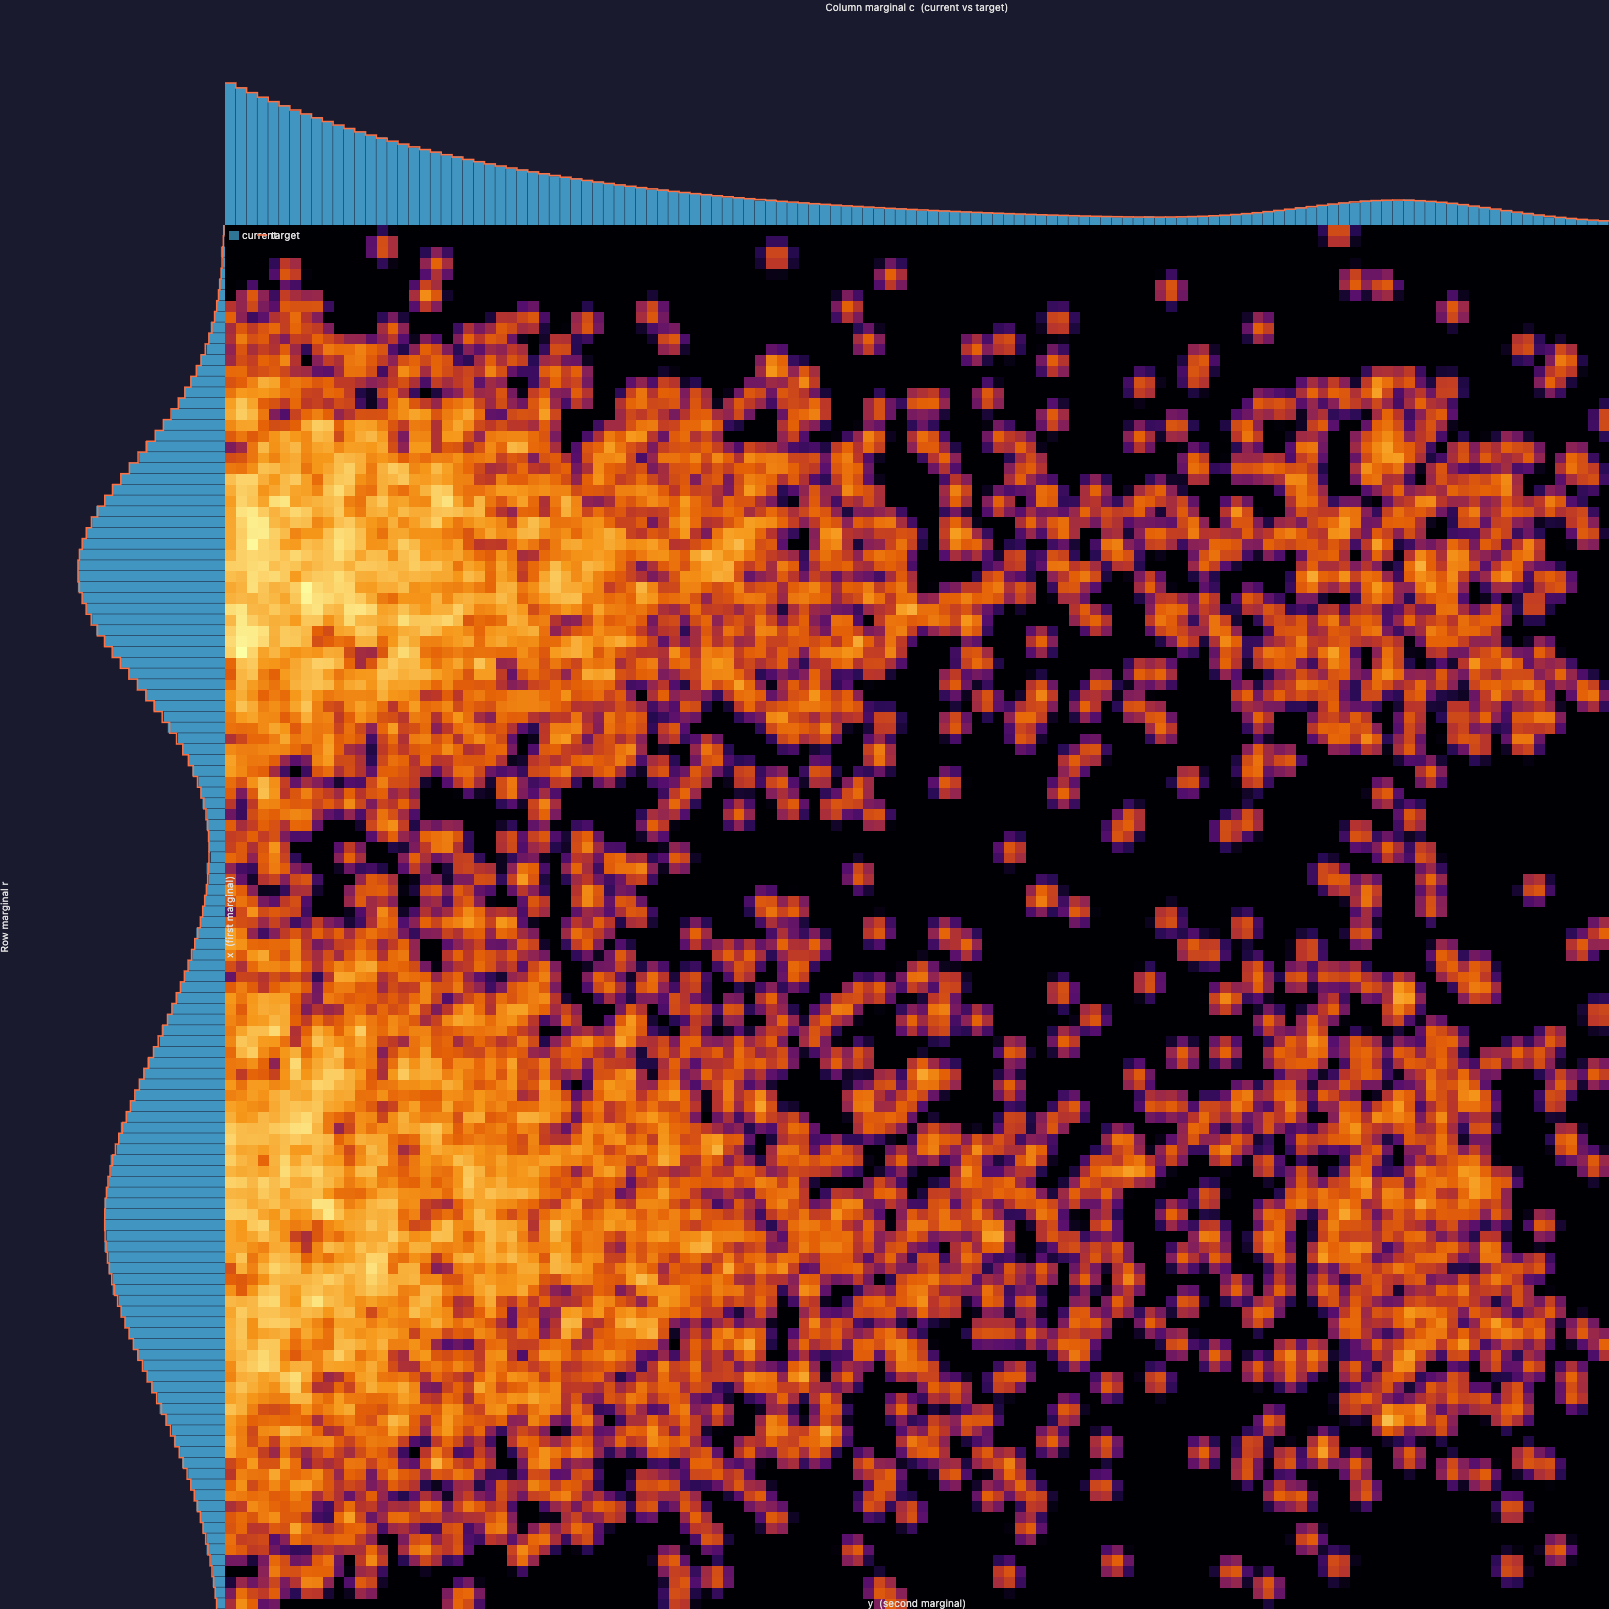
\includegraphics[width=\textwidth]{../graphics/independent.png}
        \caption{High temperature ($\varepsilon \to \infty$): maximum-entropy plan (independent coupling).}
        \label{fig:independent}
    \end{subfigure}
    \caption{Effect of the entropy regularisation parameter $\varepsilon$ on the transport plan. The heatmap shows the joint distribution of $(x, y)$ samples; marginals are shown on the axes.}
    \label{fig:epsilon_effect}
\end{figure}

\begin{algorithm}[h]
\caption{Bit-Flip MH Kernel for Regularised OT}
\label{alg:bitflip-mh}
\begin{algorithmic}[1]
\Require $M = 2^N$ particles with positions $x_1,\ldots,x_M \sim r$ and
         $y$-values $y_1,\ldots,y_M$ with empirical marginal $c$,
         regularisation $\varepsilon > 0$
\State $\mathit{bit} \gets 0$,\quad $\mathit{phase} \gets \text{y-swap}$
\Loop
    \State $\mathit{mask} \gets 2^{\mathit{bit}}$
    \For{$i = 0, 1, \ldots, M-1$ such that $(i \gg \mathit{bit}) \mathbin{\&} 1 = 0$}
        \State $j \gets i \oplus \mathit{mask}$
        \State $\Delta E \gets (x_i - y_j)^2 + (x_j - y_i)^2 - (x_i - y_i)^2 - (x_j - y_j)^2$
        \If{$\Delta E \leq 0$ \textbf{or} $U \sim \mathrm{Uniform}(0,1) < e^{-\Delta E / \varepsilon}$}
            \If{$\mathit{phase} = \text{y-swap}$} Swap $y_i \leftrightarrow y_j$
            \Else\ Swap $x_i \leftrightarrow x_j$
            \EndIf
        \EndIf
    \EndFor
    \State $\mathit{bit} \gets (\mathit{bit} + 1) \bmod N$
    \If{$\mathit{bit} = 0$} \Comment{End of full $N$-bit cycle}
        \State Shuffle particle indices
    \EndIf
\EndLoop
\end{algorithmic}
\end{algorithm}

\section{Conclusion}
In this project we have built up a deeper understanding of the Schrödinger
bridge problem based on a finite particle approach. We worked up from Brownian
bridges, to interacting particle systems to demonstrate how the KL-divergence
naturally arises as a cost-function when considering diffusion problems with
constrained marginals. Furthermore, we introduced a simple MCMC algorithm to
simulate from the posteriors defined by applying the marginal constraints to
the reference dynamics in finite particle systems. Future theoretical work
may focus on the asymptotic behaviour of such an approximation as the number of
particles increases. Of particular interest would be the relative influence of
dimensionality of the problem and number of particles on the bias term, as this
will directly impact the applicability of this method in higher dimensions.
Another open question is the best way to use more particles; i.e. whether we
should split our particles into many small systems or lump them into one larger
system. An adjacent question is what diagnostics to use for MCMC
convergence. Experimental work will explore the feasible integration of the MCMC
algorithm into diffusion modelling, including generalizing experimental results
to different forward dynamics such as the VP-SDE. It will also be of vital
interest to compare compute times with classical algorithms such as Sinkhorn and 
IPF, as well as verifying experimental outputs which to-date have been
produced by LLM's.

\appendix
\section{Experimental Results}
\label{sec:experiments}

In each table below, rows are highlighted \colorbox{yellow!40}{yellow} when the
relative bias $|\hat\mu - \mu|/|\mu|$ exceeds 10\%, \colorbox{orange!50}{orange}
when it exceeds 30\%, and \colorbox{red!40}{red} when it exceeds 50\%. Columns
shown are: dimension $d$, number of particles $M$, noise parameter
$\varepsilon$, ground truth (GT), sample mean, sample standard deviation (Std),
bias, MSE, and effective sample size (ESS). All values rounded to 4 significant
figures. There is one table per test function.

\begin{table}[htbp]
\centering
\scriptsize
\setlength{\tabcolsep}{4pt}
\begin{tabular}{rrr|rrrrrr}
\toprule
$d$ & $M$ & $\varepsilon$ & GT & Mean & Std & Bias & MSE & ESS \\
\midrule
\rowcolor{orange!50}10 & 128 & 0.05 & 0.7494 & 0.5233 & 0.002973 & -0.2261 & 0.05113 & 7.382 \\
\rowcolor{orange!50}10 & 128 & 0.1 & 0.7374 & 0.5096 & 0.00538 & -0.2278 & 0.05192 & 3.79 \\
\rowcolor{yellow!40}10 & 128 & 1.0 & 0.5693 & 0.4655 & 0.03201 & -0.1038 & 0.01179 & 332.7 \\
\midrule
\rowcolor{yellow!40}10 & 1024 & 0.05 & 0.7494 & 0.6019 & 0.001116 & -0.1475 & 0.02176 & 28.3 \\
\rowcolor{yellow!40}10 & 1024 & 0.1 & 0.7374 & 0.5967 & 0.002415 & -0.1407 & 0.0198 & 6.519 \\
\rowcolor{yellow!40}10 & 1024 & 1.0 & 0.5693 & 0.5111 & 0.01178 & -0.05823 & 0.00353 & 596.6 \\
\midrule
10 & 8192 & 0.05 & 0.7494 & 0.6947 & 0.001057 & -0.0547 & 0.002994 & 5.224 \\
10 & 8192 & 0.1 & 0.7374 & 0.6966 & 0.001954 & -0.0408 & 0.001669 & 3.964 \\
10 & 8192 & 1.0 & 0.5693 & 0.579 & 0.004242 & 0.009704 & 0.0001122 & 256.9 \\
\midrule
\rowcolor{yellow!40}30 & 128 & 0.05 & 0.7474 & 0.5666 & 7.605e-05 & -0.1808 & 0.0327 & 1000 \\
\rowcolor{orange!50}30 & 128 & 0.1 & 0.7354 & 0.3872 & 0.01337 & -0.3482 & 0.1214 & 2.94 \\
\rowcolor{yellow!40}30 & 128 & 1.0 & 0.5673 & 0.4897 & 0.02676 & -0.07763 & 0.006742 & 34.12 \\
\midrule
\rowcolor{orange!50}30 & 1024 & 0.05 & 0.7474 & 0.4653 & 0.001711 & -0.2821 & 0.07959 & 13.32 \\
\rowcolor{orange!50}30 & 1024 & 0.1 & 0.7354 & 0.4533 & 0.001838 & -0.2821 & 0.0796 & 48.23 \\
\rowcolor{yellow!40}30 & 1024 & 1.0 & 0.5673 & 0.4716 & 0.01125 & -0.09575 & 0.009295 & 15.05 \\
\midrule
\rowcolor{orange!50}30 & 8192 & 0.05 & 0.7474 & 0.5107 & 0.002323 & -0.2368 & 0.05606 & 4.919 \\
\rowcolor{orange!50}30 & 8192 & 0.1 & 0.7354 & 0.5056 & 0.001892 & -0.2298 & 0.0528 & 4.801 \\
\rowcolor{yellow!40}30 & 8192 & 1.0 & 0.5673 & 0.5065 & 0.004742 & -0.06084 & 0.003724 & 8.023 \\
\midrule
\rowcolor{red!40}100 & 128 & 0.05 & 0.7474 & 0.001647 & 0.0009059 & -0.7458 & 0.5562 & 589.2 \\
\rowcolor{red!40}100 & 128 & 0.1 & 0.7354 & 0.08254 & 0.003859 & -0.6529 & 0.4262 & 647.5 \\
\rowcolor{red!40}100 & 128 & 1.0 & 0.5673 & 0.1245 & 0.02988 & -0.4428 & 0.197 & 12.44 \\
\midrule
\rowcolor{red!40}100 & 1024 & 0.05 & 0.7474 & 0.2881 & 0.001557 & -0.4593 & 0.211 & 8.243 \\
\rowcolor{red!40}100 & 1024 & 0.1 & 0.7354 & 0.3007 & 0.001651 & -0.4347 & 0.189 & 4.214 \\
\rowcolor{orange!50}100 & 1024 & 1.0 & 0.5673 & 0.297 & 0.006806 & -0.2703 & 0.07309 & 11.6 \\
\midrule
\rowcolor{red!40}100 & 8192 & 0.05 & 0.7474 & 0.3402 & 0.002694 & -0.4073 & 0.1659 & 5.532 \\
\rowcolor{red!40}100 & 8192 & 0.1 & 0.7354 & 0.3312 & 0.002422 & -0.4042 & 0.1634 & 4.582 \\
\rowcolor{orange!50}100 & 8192 & 1.0 & 0.5673 & 0.3334 & 0.003769 & -0.2339 & 0.0547 & 7.703 \\
\bottomrule
\end{tabular}
\caption{Results for $\E(X_0^{(1)}, Y_0^{(1)})$. Rows highlighted yellow/orange/red indicate relative bias $>$10\%/30\%/50\%.}
\label{tab:x0y0}
\end{table}

\begin{table}[htbp]
\centering
\scriptsize
\setlength{\tabcolsep}{4pt}
\begin{tabular}{rrr|rrrrrr}
\toprule
$d$ & $M$ & $\varepsilon$ & GT & Mean & Std & Bias & MSE & ESS \\
\midrule
\rowcolor{yellow!40}10 & 128 & 0.05 & 0.4181 & 0.3212 & 0.003296 & -0.09692 & 0.009405 & 4.532 \\
\rowcolor{yellow!40}10 & 128 & 0.1 & 0.4179 & 0.3359 & 0.002563 & -0.08201 & 0.006733 & 4.05 \\
\rowcolor{yellow!40}10 & 128 & 1.0 & 0.392 & 0.3345 & 0.03563 & -0.05759 & 0.004586 & 485.6 \\
\midrule
10 & 1024 & 0.05 & 0.4181 & 0.4 & 0.001281 & -0.01812 & 0.00033 & 26.77 \\
10 & 1024 & 0.1 & 0.4179 & 0.3839 & 0.002224 & -0.03399 & 0.001161 & 7.58 \\
10 & 1024 & 1.0 & 0.392 & 0.3696 & 0.0128 & -0.02242 & 0.0006666 & 545.6 \\
\midrule
10 & 8192 & 0.05 & 0.4181 & 0.4357 & 0.0006305 & 0.01757 & 0.0003091 & 7.418 \\
10 & 8192 & 0.1 & 0.4179 & 0.4388 & 0.0008637 & 0.02086 & 0.0004361 & 5.173 \\
10 & 8192 & 1.0 & 0.392 & 0.4126 & 0.004755 & 0.02051 & 0.0004435 & 200.6 \\
\midrule
30 & 128 & 0.05 & 0.4159 & 0.4005 & 1.231e-05 & -0.01539 & 0.0002369 & 1000 \\
\rowcolor{orange!50}30 & 128 & 0.1 & 0.4156 & 0.2586 & 0.001127 & -0.157 & 0.02466 & 8.848 \\
\rowcolor{yellow!40}30 & 128 & 1.0 & 0.3898 & 0.3122 & 0.02284 & -0.07757 & 0.006539 & 59.98 \\
\midrule
\rowcolor{yellow!40}30 & 1024 & 0.05 & 0.4159 & 0.3432 & 0.001471 & -0.0727 & 0.005287 & 19.77 \\
\rowcolor{yellow!40}30 & 1024 & 0.1 & 0.4156 & 0.3493 & 0.003094 & -0.06636 & 0.004413 & 4.07 \\
30 & 1024 & 1.0 & 0.3898 & 0.3589 & 0.00999 & -0.0309 & 0.001055 & 32.2 \\
\midrule
30 & 8192 & 0.05 & 0.4159 & 0.3792 & 0.001021 & -0.03672 & 0.001349 & 7.193 \\
30 & 8192 & 0.1 & 0.4156 & 0.3749 & 0.001698 & -0.04076 & 0.001664 & 3.704 \\
30 & 8192 & 1.0 & 0.3898 & 0.3732 & 0.004385 & -0.0166 & 0.0002947 & 10.5 \\
\midrule
\rowcolor{red!40}100 & 128 & 0.05 & 0.4159 & -0.002341 & 0.001266 & -0.4182 & 0.1749 & 612.1 \\
\rowcolor{red!40}100 & 128 & 0.1 & 0.4156 & 0.01897 & 0.001495 & -0.3966 & 0.1573 & 623.1 \\
\rowcolor{red!40}100 & 128 & 1.0 & 0.3898 & 0.06825 & 0.02879 & -0.3215 & 0.1042 & 8.572 \\
\midrule
\rowcolor{orange!50}100 & 1024 & 0.05 & 0.4159 & 0.2507 & 0.001425 & -0.1651 & 0.02727 & 5.877 \\
\rowcolor{orange!50}100 & 1024 & 0.1 & 0.4156 & 0.2461 & 0.001548 & -0.1696 & 0.02875 & 4.861 \\
\rowcolor{orange!50}100 & 1024 & 1.0 & 0.3898 & 0.2378 & 0.006546 & -0.1519 & 0.02313 & 12.65 \\
\midrule
\rowcolor{orange!50}100 & 8192 & 0.05 & 0.4159 & 0.2763 & 0.002096 & -0.1396 & 0.01949 & 5.688 \\
\rowcolor{orange!50}100 & 8192 & 0.1 & 0.4156 & 0.274 & 0.001636 & -0.1417 & 0.02007 & 9.537 \\
\rowcolor{orange!50}100 & 8192 & 1.0 & 0.3898 & 0.2663 & 0.003044 & -0.1235 & 0.01526 & 9.918 \\
\bottomrule
\end{tabular}
\caption{Results for $\E(X_0^{(1)}, Y_1^{(1)})$. Rows highlighted yellow/orange/red indicate relative bias $>$10\%/30\%/50\%.}
\label{tab:x0y1}
\end{table}

\begin{table}[htbp]
\centering
\scriptsize
\setlength{\tabcolsep}{4pt}
\begin{tabular}{rrr|rrrrrr}
\toprule
$d$ & $M$ & $\varepsilon$ & GT & Mean & Std & Bias & MSE & ESS \\
\midrule
10 & 128 & 0.05 & 0.4181 & 0.4375 & 0.003342 & 0.01936 & 0.0003859 & 3.969 \\
10 & 128 & 0.1 & 0.4179 & 0.4456 & 0.004875 & 0.02774 & 0.0007931 & 4.358 \\
10 & 128 & 1.0 & 0.392 & 0.4301 & 0.04045 & 0.03804 & 0.003083 & 518.5 \\
\midrule
10 & 1024 & 0.05 & 0.4181 & 0.4105 & 0.001534 & -0.007662 & 6.106e-05 & 14.2 \\
10 & 1024 & 0.1 & 0.4179 & 0.4197 & 0.002937 & 0.00181 & 1.19e-05 & 6.213 \\
10 & 1024 & 1.0 & 0.392 & 0.4006 & 0.01404 & 0.008572 & 0.0002706 & 481.2 \\
\midrule
10 & 8192 & 0.05 & 0.4181 & 0.4229 & 0.0005754 & 0.00479 & 2.328e-05 & 11.5 \\
10 & 8192 & 0.1 & 0.4179 & 0.4246 & 0.0006508 & 0.006661 & 4.479e-05 & 16.93 \\
10 & 8192 & 1.0 & 0.392 & 0.4017 & 0.004994 & 0.00968 & 0.0001186 & 515.6 \\
\midrule
\rowcolor{yellow!40}30 & 128 & 0.05 & 0.4159 & 0.3462 & 0.0003115 & -0.06967 & 0.004853 & 1000 \\
\rowcolor{yellow!40}30 & 128 & 0.1 & 0.4156 & 0.366 & 0.003064 & -0.04968 & 0.002478 & 5.857 \\
\rowcolor{yellow!40}30 & 128 & 1.0 & 0.3898 & 0.4379 & 0.03565 & 0.04816 & 0.00359 & 50.94 \\
\midrule
\rowcolor{yellow!40}30 & 1024 & 0.05 & 0.4159 & 0.3605 & 0.001909 & -0.05535 & 0.003068 & 11.1 \\
30 & 1024 & 0.1 & 0.4156 & 0.4054 & 0.004868 & -0.01027 & 0.0001291 & 4.675 \\
30 & 1024 & 1.0 & 0.3898 & 0.3805 & 0.01223 & -0.009244 & 0.000235 & 32.48 \\
\midrule
\rowcolor{yellow!40}30 & 8192 & 0.05 & 0.4159 & 0.3704 & 0.0009735 & -0.04551 & 0.002072 & 6.723 \\
\rowcolor{yellow!40}30 & 8192 & 0.1 & 0.4156 & 0.3738 & 0.001458 & -0.04185 & 0.001753 & 10.16 \\
30 & 8192 & 1.0 & 0.3898 & 0.3728 & 0.003993 & -0.01703 & 0.0003059 & 30.62 \\
\midrule
\rowcolor{yellow!40}100 & 128 & 0.05 & 0.4159 & 0.4685 & 0.00298 & 0.05262 & 0.002778 & 563.2 \\
\rowcolor{yellow!40}100 & 128 & 0.1 & 0.4156 & 0.3261 & 0.006762 & -0.08957 & 0.008069 & 636.7 \\
\rowcolor{yellow!40}100 & 128 & 1.0 & 0.3898 & 0.3462 & 0.01581 & -0.04358 & 0.002149 & 10.69 \\
\midrule
\rowcolor{red!40}100 & 1024 & 0.05 & 0.4159 & 0.205 & 0.001882 & -0.2109 & 0.04447 & 122.1 \\
\rowcolor{orange!50}100 & 1024 & 0.1 & 0.4156 & 0.2383 & 0.00071 & -0.1774 & 0.03146 & 100.7 \\
\rowcolor{orange!50}100 & 1024 & 1.0 & 0.3898 & 0.2285 & 0.005915 & -0.1613 & 0.02605 & 33.44 \\
\midrule
\rowcolor{orange!50}100 & 8192 & 0.05 & 0.4159 & 0.2763 & 0.00179 & -0.1396 & 0.01948 & 5.953 \\
\rowcolor{orange!50}100 & 8192 & 0.1 & 0.4156 & 0.2769 & 0.00178 & -0.1388 & 0.01926 & 3.855 \\
\rowcolor{yellow!40}100 & 8192 & 1.0 & 0.3898 & 0.2915 & 0.00276 & -0.09824 & 0.009659 & 6.153 \\
\bottomrule
\end{tabular}
\caption{Results for $\E(X_1^{(1)}, Y_0^{(1)})$. Rows highlighted yellow/orange/red indicate relative bias $>$10\%/30\%/50\%.}
\label{tab:x1y0}
\end{table}

\begin{table}[htbp]
\centering
\scriptsize
\setlength{\tabcolsep}{4pt}
\begin{tabular}{rrr|rrrrrr}
\toprule
$d$ & $M$ & $\varepsilon$ & GT & Mean & Std & Bias & MSE & ESS \\
\midrule
\rowcolor{yellow!40}10 & 128 & 0.05 & 0.6724 & 0.5329 & 0.006668 & -0.1395 & 0.01949 & 6.802 \\
\rowcolor{yellow!40}10 & 128 & 0.1 & 0.6605 & 0.5158 & 0.002519 & -0.1448 & 0.02096 & 17.91 \\
10 & 128 & 1.0 & 0.5081 & 0.469 & 0.03568 & -0.03915 & 0.002806 & 610.2 \\
\midrule
\rowcolor{yellow!40}10 & 1024 & 0.05 & 0.6724 & 0.5441 & 0.001648 & -0.1283 & 0.01646 & 9.697 \\
\rowcolor{yellow!40}10 & 1024 & 0.1 & 0.6605 & 0.5384 & 0.002072 & -0.1221 & 0.01491 & 13.46 \\
10 & 1024 & 1.0 & 0.5081 & 0.4688 & 0.01209 & -0.03938 & 0.001697 & 640.8 \\
\midrule
10 & 8192 & 0.05 & 0.6724 & 0.6268 & 0.001809 & -0.04553 & 0.002077 & 4.363 \\
10 & 8192 & 0.1 & 0.6605 & 0.6291 & 0.00149 & -0.03142 & 0.0009892 & 5.728 \\
10 & 8192 & 1.0 & 0.5081 & 0.525 & 0.004524 & 0.01682 & 0.0003034 & 651.8 \\
\midrule
\rowcolor{red!40}30 & 128 & 0.05 & 0.6698 & 0.2422 & 5.043e-05 & -0.4277 & 0.1829 & 1000 \\
\rowcolor{red!40}30 & 128 & 0.1 & 0.658 & 0.2449 & 0.005852 & -0.413 & 0.1706 & 3.466 \\
\rowcolor{orange!50}30 & 128 & 1.0 & 0.5056 & 0.2986 & 0.03984 & -0.207 & 0.04443 & 28.13 \\
\midrule
\rowcolor{orange!50}30 & 1024 & 0.05 & 0.6698 & 0.3982 & 0.00231 & -0.2716 & 0.07379 & 8.359 \\
\rowcolor{orange!50}30 & 1024 & 0.1 & 0.658 & 0.426 & 0.004406 & -0.2319 & 0.05381 & 3.139 \\
\rowcolor{yellow!40}30 & 1024 & 1.0 & 0.5056 & 0.4125 & 0.01055 & -0.09308 & 0.008776 & 31 \\
\midrule
\rowcolor{yellow!40}30 & 8192 & 0.05 & 0.6698 & 0.4698 & 0.001152 & -0.2001 & 0.04003 & 5.967 \\
\rowcolor{yellow!40}30 & 8192 & 0.1 & 0.658 & 0.4699 & 0.002129 & -0.188 & 0.03536 & 6.008 \\
30 & 8192 & 1.0 & 0.5056 & 0.468 & 0.003233 & -0.03763 & 0.001427 & 44.49 \\
\midrule
\rowcolor{orange!50}100 & 128 & 0.05 & 0.6698 & 0.3511 & 0.003415 & -0.3187 & 0.1016 & 561.7 \\
\rowcolor{red!40}100 & 128 & 0.1 & 0.658 & 0.2607 & 0.002732 & -0.3973 & 0.1578 & 533.2 \\
\rowcolor{red!40}100 & 128 & 1.0 & 0.5056 & 0.2477 & 0.01316 & -0.2579 & 0.06669 & 12.97 \\
\midrule
\rowcolor{red!40}100 & 1024 & 0.05 & 0.6698 & 0.28 & 0.00139 & -0.3899 & 0.152 & 122.7 \\
\rowcolor{red!40}100 & 1024 & 0.1 & 0.658 & 0.3051 & 0.001088 & -0.3529 & 0.1245 & 57.87 \\
\rowcolor{orange!50}100 & 1024 & 1.0 & 0.5056 & 0.31 & 0.01162 & -0.1956 & 0.03839 & 4.518 \\
\midrule
\rowcolor{red!40}100 & 8192 & 0.05 & 0.6698 & 0.3174 & 0.002248 & -0.3524 & 0.1242 & 5.36 \\
\rowcolor{red!40}100 & 8192 & 0.1 & 0.658 & 0.3027 & 0.001761 & -0.3552 & 0.1262 & 3.494 \\
\rowcolor{orange!50}100 & 8192 & 1.0 & 0.5056 & 0.324 & 0.003875 & -0.1816 & 0.03299 & 3.202 \\
\bottomrule
\end{tabular}
\caption{Results for $\E(X_1^{(1)}, Y_1^{(1)})$. Rows highlighted yellow/orange/red indicate relative bias $>$10\%/30\%/50\%.}
\label{tab:x1y1}
\end{table}

\begin{table}[htbp]
\centering
\scriptsize
\setlength{\tabcolsep}{4pt}
\begin{tabular}{rrr|rrrrrr}
\toprule
$d$ & $M$ & $\varepsilon$ & GT & Mean & Std & Bias & MSE & ESS \\
\midrule
\rowcolor{yellow!40}10 & 128 & 0.05 & 6.698 & 5.122 & 0.004871 & -1.577 & 2.485 & 5.682 \\
\rowcolor{yellow!40}10 & 128 & 0.1 & 6.579 & 5.207 & 0.007209 & -1.373 & 1.884 & 3.366 \\
10 & 128 & 1.0 & 5.032 & 4.803 & 0.05545 & -0.2291 & 0.05554 & 661.8 \\
\midrule
\rowcolor{yellow!40}10 & 1024 & 0.05 & 6.698 & 5.608 & 0.006511 & -1.09 & 1.188 & 3.206 \\
\rowcolor{yellow!40}10 & 1024 & 0.1 & 6.579 & 5.638 & 0.007422 & -0.9415 & 0.8864 & 3.548 \\
10 & 1024 & 1.0 & 5.032 & 4.881 & 0.0231 & -0.1511 & 0.02337 & 373.5 \\
\midrule
10 & 8192 & 0.05 & 6.698 & 6.099 & 0.01337 & -0.5995 & 0.3596 & 4.386 \\
10 & 8192 & 0.1 & 6.579 & 6.111 & 0.01685 & -0.4681 & 0.2194 & 3.789 \\
10 & 8192 & 1.0 & 5.032 & 5.057 & 0.008552 & 0.02469 & 0.0006828 & 479.1 \\
\midrule
\rowcolor{orange!50}30 & 128 & 0.05 & 19.11 & 10.15 & 5.227e-05 & -8.966 & 80.39 & 1000 \\
\rowcolor{orange!50}30 & 128 & 0.1 & 18.76 & 10.11 & 0.03396 & -8.648 & 74.79 & 3.004 \\
\rowcolor{yellow!40}30 & 128 & 1.0 & 14.19 & 10.37 & 0.03395 & -3.819 & 14.59 & 16.18 \\
\midrule
\rowcolor{orange!50}30 & 1024 & 0.05 & 19.11 & 11.92 & 0.008247 & -7.19 & 51.7 & 7.456 \\
\rowcolor{orange!50}30 & 1024 & 0.1 & 18.76 & 11.99 & 0.01975 & -6.767 & 45.79 & 2.689 \\
\rowcolor{yellow!40}30 & 1024 & 1.0 & 14.19 & 12.18 & 0.02637 & -2.015 & 4.062 & 10.88 \\
\midrule
\rowcolor{orange!50}30 & 8192 & 0.05 & 19.11 & 13.26 & 0.04017 & -5.855 & 34.29 & 5.442 \\
\rowcolor{yellow!40}30 & 8192 & 0.1 & 18.76 & 13.28 & 0.04502 & -5.477 & 30 & 4.405 \\
30 & 8192 & 1.0 & 14.19 & 13.25 & 0.05461 & -0.9404 & 0.8874 & 4.671 \\
\midrule
\rowcolor{red!40}100 & 128 & 0.05 & 62.55 & 20.31 & 0.0001763 & -42.24 & 1784 & 580 \\
\rowcolor{red!40}100 & 128 & 0.1 & 61.37 & 20.42 & 0.0002096 & -40.95 & 1677 & 640.4 \\
\rowcolor{red!40}100 & 128 & 1.0 & 46.25 & 20.78 & 0.09664 & -25.47 & 648.8 & 7.634 \\
\midrule
\rowcolor{red!40}100 & 1024 & 0.05 & 62.55 & 24.99 & 0.009646 & -37.56 & 1411 & 4.077 \\
\rowcolor{red!40}100 & 1024 & 0.1 & 61.37 & 24.98 & 0.00768 & -36.39 & 1324 & 3.547 \\
\rowcolor{orange!50}100 & 1024 & 1.0 & 46.25 & 25.63 & 0.102 & -20.62 & 425.3 & 4.453 \\
\midrule
\rowcolor{red!40}100 & 8192 & 0.05 & 62.55 & 28.39 & 0.09608 & -34.16 & 1167 & 5.486 \\
\rowcolor{red!40}100 & 8192 & 0.1 & 61.37 & 28.39 & 0.09716 & -32.98 & 1088 & 5.422 \\
\rowcolor{orange!50}100 & 8192 & 1.0 & 46.25 & 28.9 & 0.2425 & -17.35 & 301.1 & 3.714 \\
\bottomrule
\end{tabular}
\caption{Results for $\mathbb{E}[X \cdot Y]$. Rows highlighted yellow/orange/red indicate relative bias $>$10\%/30\%/50\%.}
\label{tab:EZ}
\end{table}

\begin{table}[htbp]
\centering
\scriptsize
\setlength{\tabcolsep}{4pt}
\begin{tabular}{rrr|rrrrrr}
\toprule
$d$ & $M$ & $\varepsilon$ & GT & Mean & Std & Bias & MSE & ESS \\
\midrule
\rowcolor{orange!50}10 & 128 & 0.05 & 65.7 & 41.21 & 0.0799 & -24.49 & 599.9 & 5.693 \\
\rowcolor{orange!50}10 & 128 & 0.1 & 63.96 & 41.9 & 0.09582 & -22.06 & 486.6 & 3.203 \\
\rowcolor{yellow!40}10 & 128 & 1.0 & 43.81 & 38.85 & 0.665 & -4.964 & 25.09 & 427 \\
\midrule
\rowcolor{yellow!40}10 & 1024 & 0.05 & 65.7 & 47.25 & 0.09018 & -18.45 & 340.4 & 3.81 \\
\rowcolor{yellow!40}10 & 1024 & 0.1 & 63.96 & 47.65 & 0.1089 & -16.31 & 266 & 3.634 \\
10 & 1024 & 1.0 & 43.81 & 40.63 & 0.312 & -3.177 & 10.19 & 230.7 \\
\midrule
\rowcolor{yellow!40}10 & 8192 & 0.05 & 65.7 & 55.93 & 0.1793 & -9.773 & 95.54 & 4.491 \\
\rowcolor{yellow!40}10 & 8192 & 0.1 & 63.96 & 56.18 & 0.2181 & -7.78 & 60.57 & 3.765 \\
10 & 8192 & 1.0 & 43.81 & 44.84 & 0.1297 & 1.026 & 1.07 & 90.22 \\
\midrule
\rowcolor{red!40}30 & 128 & 0.05 & 425.8 & 130 & 0.002421 & -295.8 & 8.748e+04 & 1000 \\
\rowcolor{red!40}30 & 128 & 0.1 & 411.9 & 130.8 & 0.5947 & -281 & 7.898e+04 & 3.425 \\
\rowcolor{orange!50}30 & 128 & 1.0 & 255.4 & 135.5 & 0.7852 & -119.9 & 1.437e+04 & 9.689 \\
\midrule
\rowcolor{red!40}30 & 1024 & 0.05 & 425.8 & 176.9 & 0.1732 & -248.9 & 6.196e+04 & 7.986 \\
\rowcolor{red!40}30 & 1024 & 0.1 & 411.9 & 179 & 0.4563 & -232.9 & 5.424e+04 & 2.685 \\
\rowcolor{yellow!40}30 & 1024 & 1.0 & 255.4 & 184.8 & 0.7381 & -70.56 & 4979 & 9.279 \\
\midrule
\rowcolor{orange!50}30 & 8192 & 0.05 & 425.8 & 215.3 & 0.9978 & -210.5 & 4.431e+04 & 5.585 \\
\rowcolor{orange!50}30 & 8192 & 0.1 & 411.9 & 216.5 & 1.248 & -195.4 & 3.818e+04 & 4.501 \\
\rowcolor{yellow!40}30 & 8192 & 1.0 & 255.4 & 218.4 & 1.595 & -36.98 & 1370 & 4.259 \\
\midrule
\rowcolor{red!40}100 & 128 & 0.05 & 4112 & 458.4 & 0.1763 & -3654 & 1.335e+07 & 569.6 \\
\rowcolor{red!40}100 & 128 & 0.1 & 3964 & 462.3 & 0.2373 & -3501 & 1.226e+07 & 644.9 \\
\rowcolor{red!40}100 & 128 & 1.0 & 2317 & 476.6 & 3.211 & -1840 & 3.387e+06 & 10.18 \\
\midrule
\rowcolor{red!40}100 & 1024 & 0.05 & 4112 & 693.3 & 0.5409 & -3419 & 1.169e+07 & 4.628 \\
\rowcolor{red!40}100 & 1024 & 0.1 & 3964 & 692.8 & 0.3602 & -3271 & 1.07e+07 & 3.591 \\
\rowcolor{red!40}100 & 1024 & 1.0 & 2317 & 725.9 & 4.609 & -1591 & 2.531e+06 & 4.421 \\
\midrule
\rowcolor{red!40}100 & 8192 & 0.05 & 4112 & 886.4 & 5.099 & -3226 & 1.041e+07 & 5.455 \\
\rowcolor{red!40}100 & 8192 & 0.1 & 3964 & 886.4 & 5.133 & -3077 & 9.47e+06 & 5.49 \\
\rowcolor{red!40}100 & 8192 & 1.0 & 2317 & 916.9 & 13.57 & -1400 & 1.96e+06 & 3.665 \\
\bottomrule
\end{tabular}
\caption{Results for $\mathbb{E}[(X \cdot Y)^2]$. Rows highlighted yellow/orange/red indicate relative bias $>$10\%/30\%/50\%.}
\label{tab:EZ2}
\end{table}

\begin{table}[htbp]
\centering
\scriptsize
\setlength{\tabcolsep}{4pt}
\begin{tabular}{rrr|rrrrrr}
\toprule
$d$ & $M$ & $\varepsilon$ & GT & Mean & Std & Bias & MSE & ESS \\
\midrule
\rowcolor{orange!50}10 & 128 & 0.05 & 899.1 & 456.7 & 0.8787 & -442.4 & 1.957e+05 & 5.727 \\
\rowcolor{orange!50}10 & 128 & 0.1 & 871.2 & 463.9 & 1.171 & -407.3 & 1.659e+05 & 3.337 \\
\rowcolor{yellow!40}10 & 128 & 1.0 & 561 & 434.5 & 11.96 & -126.5 & 1.615e+04 & 308.9 \\
\midrule
\rowcolor{orange!50}10 & 1024 & 0.05 & 899.1 & 552.4 & 1.498 & -346.7 & 1.202e+05 & 4.921 \\
\rowcolor{orange!50}10 & 1024 & 0.1 & 871.2 & 561.9 & 2.6 & -309.3 & 9.567e+04 & 3.935 \\
\rowcolor{yellow!40}10 & 1024 & 1.0 & 561 & 483 & 7.052 & -78.04 & 6139 & 143.6 \\
\midrule
\rowcolor{yellow!40}10 & 8192 & 0.05 & 899.1 & 733.9 & 2.857 & -165.2 & 2.73e+04 & 4.421 \\
\rowcolor{yellow!40}10 & 8192 & 0.1 & 871.2 & 739.1 & 3.024 & -132.1 & 1.746e+04 & 3.6 \\
10 & 8192 & 1.0 & 561 & 598.2 & 3.335 & 37.18 & 1394 & 36.81 \\
\midrule
\rowcolor{red!40}30 & 128 & 0.05 & 1.107e+04 & 1998 & 0.04142 & -9074 & 8.233e+07 & 1000 \\
\rowcolor{red!40}30 & 128 & 0.1 & 1.059e+04 & 2043 & 8.111 & -8551 & 7.312e+07 & 4.268 \\
\rowcolor{red!40}30 & 128 & 1.0 & 5700 & 2117 & 19.94 & -3583 & 1.284e+07 & 10.31 \\
\midrule
\rowcolor{red!40}30 & 1024 & 0.05 & 1.107e+04 & 3184 & 3.509 & -7888 & 6.222e+07 & 9.2 \\
\rowcolor{red!40}30 & 1024 & 0.1 & 1.059e+04 & 3239 & 10.91 & -7354 & 5.409e+07 & 2.785 \\
\rowcolor{orange!50}30 & 1024 & 1.0 & 5700 & 3388 & 21.66 & -2312 & 5.347e+06 & 15.45 \\
\midrule
\rowcolor{red!40}30 & 8192 & 0.05 & 1.107e+04 & 4211 & 22.17 & -6861 & 4.707e+07 & 5.743 \\
\rowcolor{red!40}30 & 8192 & 0.1 & 1.059e+04 & 4267 & 32.71 & -6327 & 4.003e+07 & 4.628 \\
\rowcolor{yellow!40}30 & 8192 & 1.0 & 5700 & 4358 & 41.67 & -1342 & 1.803e+06 & 4.103 \\
\midrule
\rowcolor{red!40}100 & 128 & 0.05 & 2.843e+05 & 1.138e+04 & 8.229 & -2.73e+05 & 7.451e+10 & 574.8 \\
\rowcolor{red!40}100 & 128 & 0.1 & 2.697e+05 & 1.142e+04 & 14.46 & -2.583e+05 & 6.671e+10 & 635.1 \\
\rowcolor{red!40}100 & 128 & 1.0 & 1.255e+05 & 1.197e+04 & 104.8 & -1.136e+05 & 1.29e+10 & 19.54 \\
\midrule
\rowcolor{red!40}100 & 1024 & 0.05 & 2.843e+05 & 2.116e+04 & 25.97 & -2.632e+05 & 6.926e+10 & 5.761 \\
\rowcolor{red!40}100 & 1024 & 0.1 & 2.697e+05 & 2.11e+04 & 13.39 & -2.486e+05 & 6.18e+10 & 3.686 \\
\rowcolor{red!40}100 & 1024 & 1.0 & 1.255e+05 & 2.254e+04 & 164.3 & -1.03e+05 & 1.061e+10 & 4.627 \\
\midrule
\rowcolor{red!40}100 & 8192 & 0.05 & 2.843e+05 & 3.024e+04 & 223.9 & -2.541e+05 & 6.457e+10 & 5.452 \\
\rowcolor{red!40}100 & 8192 & 0.1 & 2.697e+05 & 3.028e+04 & 227 & -2.394e+05 & 5.732e+10 & 5.542 \\
\rowcolor{red!40}100 & 8192 & 1.0 & 1.255e+05 & 3.174e+04 & 636.1 & -9.38e+04 & 8.799e+09 & 3.597 \\
\bottomrule
\end{tabular}
\caption{Results for $\mathbb{E}[(X \cdot Y)^3]$. Rows highlighted yellow/orange/red indicate relative bias $>$10\%/30\%/50\%.}
\label{tab:EZ3}
\end{table}

\bibliographystyle{plain}
\bibliography{refs}


\end{document}